\section{PROCEDIMENTO EXPERIMENTAL}

\subsection{Materiais}

\begin{itemize}
    \item Inserir materiais.
\end{itemize}

\subsection{Metodologia}

Inserir texto. Exemplo de figura e de citação de figura no texto: Figura (\ref{fCil}).

\begin{figure}[H]
    \centering
    \caption{Cilindro polimérico utilizado no experimento}
    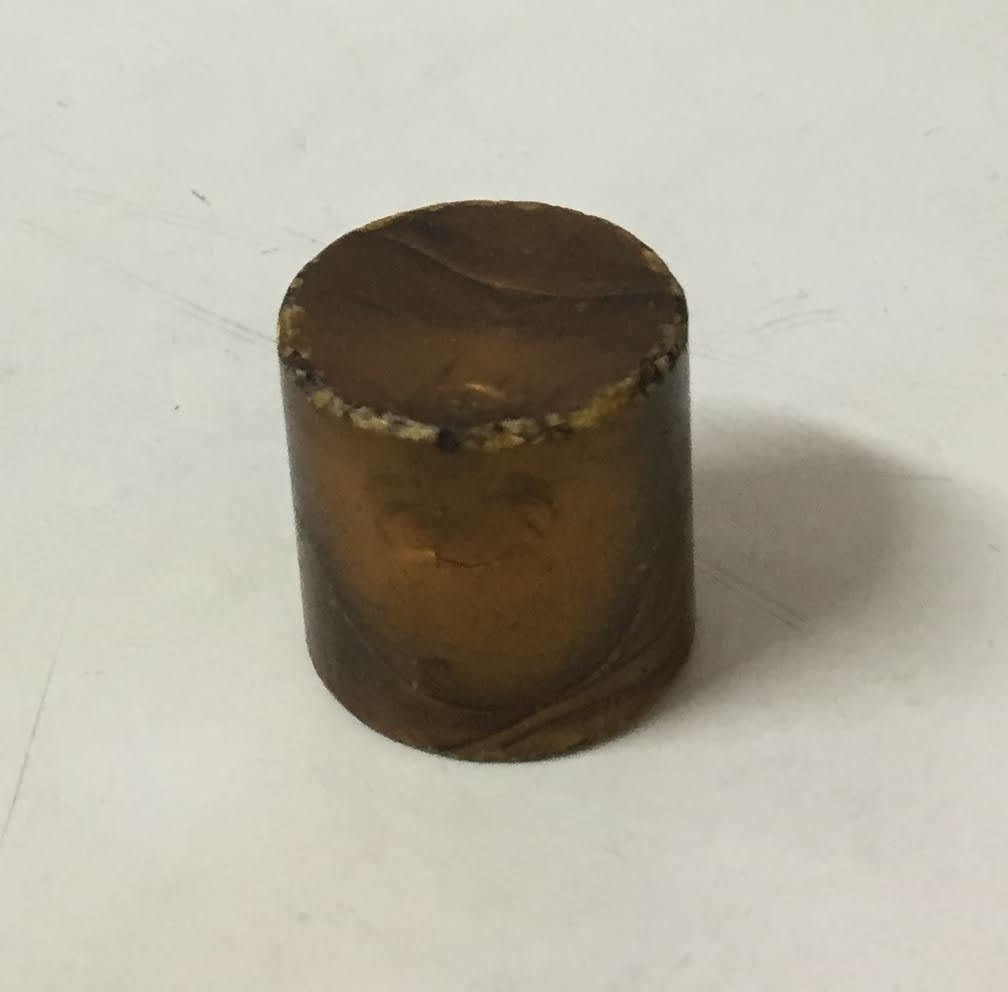
\includegraphics{Figuras/Figura 01.JPG}\\
    \autoria
    \label{fCil}
\end{figure}


\subsection{Medições}

Inserir texto. Exemplo de tabela e citação de tabela: tabela (\ref{tCilPaq}).

% Tabela de Dimensões do Cilindro
\begin{table}[H]
\centering
\caption{Medições das dimensões do cilindro realizadas com o paquímetro.}
\label{tCilPaq}
\begin{tabular}{ccc}
\hline
Medidas (i) & Altura (mm) & Diâmetro(mm)\\
\hline
1 & 24,55 & 24,65 \\
2 & 24,60 & 24,65 \\
3 & 24,45 & 24,75 \\
4 & 24,45 & 24,65 \\
5 & 24,60 & 24,75 \\
6 & 24,60 & 24,5 \\
7 & 24,60 & 24,7 \\
8 & 24,60 & 24,65 \\
9 & 24,60 & 24,65 \\
10 & 24,60 & 24,5\\
\hline
\end{tabular}\\
\autoria
\end{table}